\documentclass[12pt,a4paper]{article}

\usepackage{graphicx}% Include figure files
\usepackage{dcolumn}% Align table columns on decimal point
\usepackage{bm}% bold math
%\usepackage{hyperref}% add hypertext capabilities
%\usepackage[mathlines]{lineno}% Enable numbering of text and display math
%\linenumbers\relax % Commence numbering lines

%\usepackage[showframe,%Uncomment any one of the following lines to test 
%%scale=0.7, marginratio={1:1, 2:3}, ignoreall,% default settings
%%text={7in,10in},centering,
%%margin=1.5in,
%%total={6.5in,8.75in}, top=1.2in, left=0.9in, includefoot,
%%height=10in,a5paper,hmargin={3cm,0.8in},
%]{geometry}

\usepackage{multicol}%Para hacer varias columnas
\usepackage{multicol,caption}
\usepackage{multirow}
\usepackage{cancel}
\usepackage{hyperref}
\hypersetup{
    colorlinks=true,
    linkcolor=blue,
    filecolor=magenta,      
    urlcolor=cyan,
}

\setlength{\topmargin}{-1.0in}
\setlength{\oddsidemargin}{-0.3pc}
\setlength{\evensidemargin}{-0.3pc}
\setlength{\textwidth}{6.75in}
\setlength{\textheight}{9.5in}
\setlength{\parskip}{0.5pc}

\usepackage[utf8]{inputenc}
\usepackage{expl3,xparse,xcoffins,titling,kantlipsum}
\usepackage{graphicx}
\usepackage{xcolor} 
\usepackage{siunitx}
\usepackage{nopageno}
\usepackage{lettrine}
\usepackage{caption}
\renewcommand{\figurename}{Figura}
\usepackage{float}
\renewcommand\refname{Bibliograf\'ia}
\usepackage{amssymb}
\usepackage{amsmath}
\usepackage[rightcaption]{sidecap}
\usepackage[spanish]{babel}

\providecommand{\abs}[1]{\lvert#1\rvert}
\providecommand{\norm}[1]{\lVert#1\rVert}
\newcommand{\dbar}{\mathchar'26\mkern-12mu d}

% CABECERA Y PIE DE PÁGINA %%%%%
\usepackage{fancyhdr}
\pagestyle{fancy}
\fancyhf{}

\begin{document}

Macías Márquez Misael Iván

\begin{enumerate}



%%%1%%%



    \item Muestre que el calor transferido durante un proceso cuasi-estático infinitesimal de un gas ideal puede escribirse como:
    
    
    \begin{equation*}
        \dbar Q = \frac{C_V}{nR} VdP + \frac{C_P}{nR} PdV 
    \end{equation*}
    
    aplicando esta ecuación a un proceso adiabático muestre que
    
    \begin{equation*}
        PV^\gamma = constante
    \end{equation*}
    
    \textbf{Sol:}
    
     La relación de la tarea anterior es 
     
     \begin{equation*}
         \dbar Q = C_P d\theta - \frac{\kappa_\theta}{\beta}(C_P - C_V) dP
     \end{equation*}
    
    y como tenemos un gas ideal, $\kappa_\theta = \frac{1}{p}$, $\beta = \frac{1}{\theta}$, por lo que $\frac{\kappa_\theta}{\beta} = \frac{\theta}{p}$ o bien despejando en la ec. del gas ideal, $\frac{\kappa_\theta}{\beta} = \frac{V}{nR}$, entonces
    
    \begin{equation*}
         \dbar Q = C_P( d\theta - \frac{\theta}{p}dP)+ C_V\frac{V}{nR} dP
     \end{equation*}
     
     ahora si $P$ es constante y derivando la ec. del gas ideal, $d \theta = \frac{P}{nR}dV$ y $dP = 0$
     
     \begin{equation*}
         \dbar Q = C_P( \frac{P}{nR} dV - \cancel{\frac{\theta}{p}dP})+ C_V\frac{V}{nR} dP = C_P \frac{P}{nR} dV+ C_V\frac{V}{nR} dP
     \end{equation*}
     
     para lo siguiente, como es un proceso adiabático, entonces
     
     \begin{equation*}
         0 =C_P \frac{P}{nR} dV+ C_V\frac{V}{nR} dP
     \end{equation*}
     
     \begin{equation*}
         -  \frac{dP}{P}= \gamma \frac{dV}{V}
     \end{equation*}
     
     \begin{equation*}
        -\int \frac{d P}{P} =\gamma \int \frac{dV}{V} 
     \end{equation*}
     
     \begin{equation*}
         -\ln{P} =  \gamma \ln{V} + c
     \end{equation*}
     
     \begin{equation*}
         \ln{P}+\ln{V^{\gamma}} =  \ln{PV^{\gamma}}= k
     \end{equation*}
     
     \begin{equation*}
         P V^{\gamma} = k' = cte
     \end{equation*}
     
     
    
%%%2%%%
    
    
    
    \item Muestre que el trabajo realizado por un gas ideal con capacidades caloríficas constantes durante una expansión cuasi-estática adiabática es igual a:
    
    \begin{enumerate}
        \item $W = C_V (T_f - T_i)$
        
        \textbf{Sol:}
        
        Por la primera ley y como es un proceso adiabático
        
        \begin{equation*}
            \cancel{\dbar} = dU - dW \hspace{1cm} \rightarrow \hspace{1cm} dW = dU = C_V (T_f - T_i) 
        \end{equation*}
        
        
        \item $W = \frac{P_f V_f - P_i V_i}{1-\gamma}$
        
        \textbf{Sol:}
        
        Por el ejercicio 1,
        
        \begin{equation*}
            W = \int_{V_i}^{V_f} PdV = c \int_{V_i}^{V_f} \frac{dV}{V^{\gamma}} = c\frac{(V_{f}^{\gamma - 1} - V_{i} ^{\gamma - 1})}{\gamma - 1}
        \end{equation*}
        
        pero $PV = c V^{\gamma - 1}$
        
        \begin{equation*}
            W =  \frac{P_{f} V_{f} - P_{i}V_{i}}{\gamma - 1}
        \end{equation*}
        
        
        \item $W = \frac{P_f V_f}{\gamma - 1}\left[1 - \left(\frac{P_i}{P_f}\right)^{(\gamma - 1)/\gamma}\right]$
        
        \textbf{Sol:}
        
        Por el b)
        
        \begin{equation*}
            W =  \frac{P_{f} V_{f} - P_{i}V_{i}}{\gamma - 1} = \frac{P_{f} V_{f} - \frac{P_{i}V_{i}^{\gamma}}{V_{i}^{\gamma - 1}}}{\gamma - 1} 
        \end{equation*}
        
        y por ser un gas ideal ( $P_i V_{i}^{\gamma} = P_{f} V_{f}^{\gamma}$)
        
        \begin{equation*}
            W =\frac{P_{f} V_{f} - \frac{P_{f}V_{f}^{\gamma}}{V_{i}^{\gamma - 1}}}{\gamma - 1} = \frac{P_f V_f}{\gamma - 1} \left[ 1 - \frac{V_{f}^{\gamma - 1}}{V_{i}^{\gamma - 1}}\right] = \frac{P_f V_f}{\gamma - 1}\left[1 - \left(\frac{P_i}{P_f}\right)^{(\gamma - 1)/\gamma}\right]
        \end{equation*}
        
    \end{enumerate}
    
    
    
%%%3%%%
    
    
    
    \item Derive la siguiente fórmula para un proceso cuasi-estático adiabático para el gas ideal, considere $\gamma = cte$
    
    \begin{equation*}
        TV^{\gamma -1} = cte
    \end{equation*}
    
    \textbf{Sol:}
    
    por el ejercicio 1
    
    \begin{equation*}
        PV^{\gamma} = c
    \end{equation*}
    
    \begin{equation*}
        PV^{\gamma - 1 + 1} = c
    \end{equation*}
    
    \begin{equation*}
        PV V^{\gamma - 1} = c
    \end{equation*}
    
    y como $PV = nR T$
    
    \begin{equation*}
        nR T V^{\gamma - 1} = c
    \end{equation*}
    
    \begin{equation*}
        T V^{\gamma - 1} = \frac{c}{nR} = c' = cte 
    \end{equation*}
    

    
    
    
%%%4%%%
    
    
    
    \item Imagine que trabaja en una oficina de patentes, una compañía presenta un examen de patente para una máquina térmica cuya eficiencia -afirma- es del 75\%, la máquina funciona entre 2 baños térmicos de $20^{\cdot} C$ y $800^{\cdot}C$. En cada ciclo la máquina realiza un trabajo de $30,000 $ J, disipando $10, 000$ J al baño frío. ¿Otorgaría la patente?. Justifique su respuesta.
    
    \textbf{Sol:}
    
    Suponiendo que esta máquina es la más eficiente posible (máquina de Carnot) entonces la eficiencia sería
    
    \begin{equation*}
        \eta = 1 - \frac{T_C}{T_H} = 1 - \frac{296.15 K}{1073.15 K} = 0.724 = 72.4 \%
    \end{equation*}
    
    por lo que no sería posible la eficiencia que declaran aunque su máquina sea 'perfecta'.
    
    Ahora el trabajo realizado y disipado nos da una eficiencia de
    
    \begin{equation*}
        \eta = 1 - \frac{10000 J}{30000 J} = 0.667 = 66.7 \%
    \end{equation*}
    
    entonces creo que no se daría la patente.
    
    
    
%%%5%%%
    
    
    
    \item Considere una máquina trabajando en un ciclo reversible y que emplea un gas ideal de capacidad calorífica $C_p$ como sustancia que trabaja. El ciclo consiste de dos procesos a presión constante, conectados por dos adiabáticas (figura 1).
    
    \begin{enumerate}
        \item Encuentre la eficiencia de esta máquina en términos de $P_1$ y $P_2$.
        
        \textbf{Sol:}
        
        Como los procesos $BC$ y $DA$ son adiabáticos, no se tiene transferencia de calor, así que esta se debe dar en los procesos $AB$ y $CD$, el trabajo para ambos procesos es
        
        \begin{equation*}
            W = P_i\int d V = P_i \Delta V 
        \end{equation*}
        
        y como se emplea un gas ideal
        
        \begin{equation*}
          W = nR \Delta T   
        \end{equation*}
        
        también sabemos que la energía interna está determinada por
        
        \begin{equation*}
            U = C_V \Delta T \hspace{2cm} \therefore Q = \Delta T (C_V + nR) = \Delta T C_P
        \end{equation*}
        
        o bien $Q = C_P P_i \Delta V /nR$, y entonces la eficiencia es (suponiendo que $|\Delta V |_{AB} = |\Delta V| _{CD}$)
        
        \begin{equation*}
            \eta = 1 - \frac{|Q_H|}{|Q_C|} = 1 -  \frac{P_2}{P_1} \cancel{\frac{nR |\Delta V|_{CD}}{nR |\Delta V|_{AB}}} = 1 - \frac{P_2}{P_1}
        \end{equation*}
        
        \item ¿Cuál de las temperaturas $T_A$, $T_B$, $T_C$, $T_D$ es la más alta?, ¿Cuál es la más baja?
        
        \textbf{Sol:}
        
        Como tenemos un gas ideal, entonces $T = \frac{PV}{nR}$ y como $nR$ son contantes, $T_{max} = \frac{P_B V_B}{nR} = T_B$ y $T_{min} = \frac{P_D V_D}{nR} = T_D$ 
        
        \item Como se compara esta máquina con una de Carnot trabajando con el mismo gas entre las temperaturas mas baja y más alta?
        
        \textbf{Sol:}
        
        Ya que $P = \frac{TnR}{V}$ para un gas ideal, entonces
        
        \begin{equation*}
            \eta = 1 - \frac{P_2}{P_1} = 1 - \frac{T_2}{T_1} \frac{V_1}{V_2}
        \end{equation*}
        
        y como $V_1 > V_2$ por lo  que su eficiencia es menor a la de Carnot
        
    \end{enumerate}
    
    \begin{figure}[h!]
        \centering
        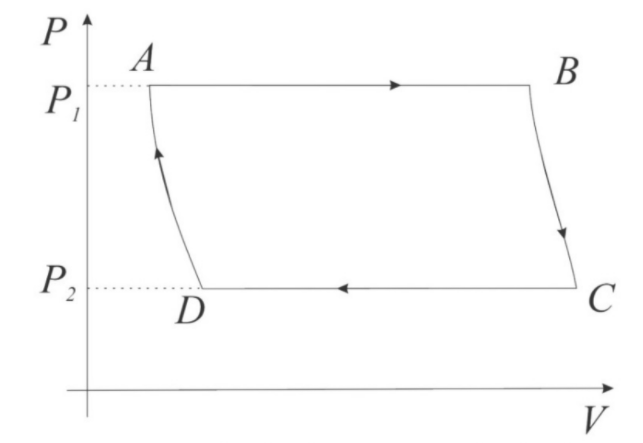
\includegraphics[scale = 0.8]{1.PNG}
    \end{figure}
    
    
\end{enumerate}

\end{document}

